% !TEX program = xelatex
\documentclass[a4paper,14pt,oneside,openany]{memoir}

%%% Задаем поля, отступы и межстрочный интервал %%%

\usepackage[left=30mm, right=15mm, top=20mm, bottom=20mm]{geometry}
\pagestyle{plain}
\parindent=1.25cm
\usepackage{indentfirst}

%%% Задаем языковые параметры и шрифт %%%

\usepackage[english,russian]{babel}
\babelfont[russian]{rm}{Times New Roman}
\babelfont[russian]{tt}{Courier New}

%%% Задаем стиль заголовков и подзаголовков в тексте %%%

\setsecnumdepth{subsection}
\renewcommand*{\chapterheadstart}{}
\renewcommand*{\printchaptername}{}
\renewcommand*{\chapnumfont}{\normalfont\bfseries}
\renewcommand*{\afterchapternum}{\hspace{1em}}
\renewcommand*{\printchaptertitle}{\normalfont\bfseries\centering\MakeUppercase}
\setbeforesecskip{20pt}
\setaftersecskip{20pt}
\setsecheadstyle{\raggedright\normalfont\bfseries}
\setbeforesubsecskip{20pt}
\setaftersubsecskip{20pt}
\setsubsecheadstyle{\raggedright\normalfont\bfseries}

%%% Исправление нумерации секций %%%

\renewcommand{\thesection}{\arabic{section}}
\renewcommand{\thesubsection}{\arabic{subsection}}

%%% Сквозная нумерация рисунков и таблиц %%%

\counterwithout{figure}{chapter}
\counterwithout{table}{chapter}

%%% Выравнивание и переносы %%%

\tolerance 1414
\hbadness 1414
\emergencystretch 1.5em
\clubpenalty=10000
\widowpenalty=10000

%%% Задаем параметры оформления рисунков и таблиц %%%

\usepackage{graphicx}
\usepackage{caption}
\usepackage{subcaption}
\usepackage{float}
\graphicspath{{photo/}}
\captionsetup[figure]{font=small, width=\textwidth, name=Рисунок, justification=centering}
\captiondelim{ --- }
\usepackage[section]{placeins}

%%% Задаем параметры ссылок и гиперссылок %%% 

\usepackage{hyperref}
\hypersetup{
    colorlinks=true,
    linkcolor=red,
    citecolor=red
}

%%% Настраиваем отображение списков %%%

\usepackage{enumitem}
\renewcommand*{\labelitemi}{\normalfont{--}}
\setlist{noitemsep, leftmargin=*}

\begin{document}

% Титульный лист (без номера страницы)
\thispagestyle{empty}

\begin{center}
    МИНИСТЕРСТВО ЦИФРОВОГО РАЗВИТИЯ, СВЯЗИ И МАССОВЫХ \\ КОММУНИКАЦИЙ \\ РОССИЙСКОЙ ФЕДЕРАЦИИ

    \vspace{20pt}

    Федеральное государственное бюджетное образовательное учреждение \\ высшего образования \\
    "Сибирский государственный университет телекоммуникаций и \\ информатики"

    \vspace{20pt}

    Кафедра телекоммуникационных систем и вычислительных средств \\ (ТС и ВС)
\end{center}

\vfill

\begin{center}
    Практическая работа №11 \\
    по дисциплине \\
    \textit{"Web-технологии"}

    \vspace{20pt}

    по теме: \\
    \uppercase{Веб-дизайн}
\end{center}

\vfill

\noindent Студент: \\
\textit{Группа ИКС-532 \hfill А.С. Лёшин}

\vspace{20pt}

\noindent Преподаватель: \\
\textit{старший преподаватель \hfill А.В. Андреев}

\vfill

\begin{center}
    Новосибирск 2026 г.
\end{center}

\newpage
\setcounter{page}{2}
\OnehalfSpacing*

\subsection*{Цель работы}

\begin{itemize}
    \item Разработать дизайн-концепцию сайта чемпионата по фиджитал-спорту (кибер-гольф)
    \item Создать адаптивный макет для ПК, планшета и мобильных устройств
    \item Реализовать 5 обязательных страниц: главная, команда, участник, турнирная таблица, каталог сувениров
    \item Добавить коммерческую поддержку (продажа билетов с дегустацией, продажа сувениров)
    \item Обеспечить спортивно-информационное освещение мероприятия
\end{itemize}

\section{Введение}

Фиджитал-спорт — это новый вид соревнований, объединяющий физическую активность и цифровую среду. В рамках данной работы был разработан сайт чемпионата по кибер-гольфу "Кубок Сибири 2024", который пройдёт в Новосибирске с 15 по 18 октября.

Сайт выполняет три основные функции:
\begin{enumerate}
    \item Спортивно-информационное обеспечение (список команд, турнирная таблица, карточки участников)
    \item Информационное освещение (новости, место проведения)
    \item Коммерческая поддержка (продажа билетов с возможностью выбора типа, продажа сувенирной продукции)
\end{enumerate}

\section{Результаты выполнения}

Ниже представлены скриншоты разработанного макета сайта чемпионата по кибер-гольфу.

\begin{figure}[H]
    \centering
    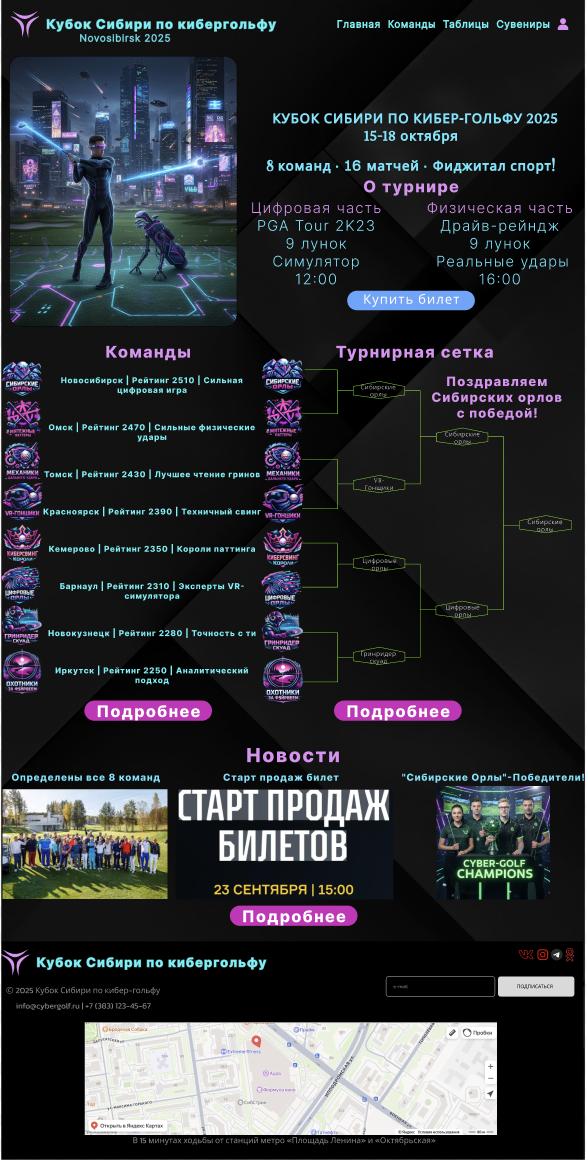
\includegraphics[width=0.7\textwidth]{photo/1.png}
    \caption{Главная страница}
\end{figure}

\begin{figure}[H]
    \centering
    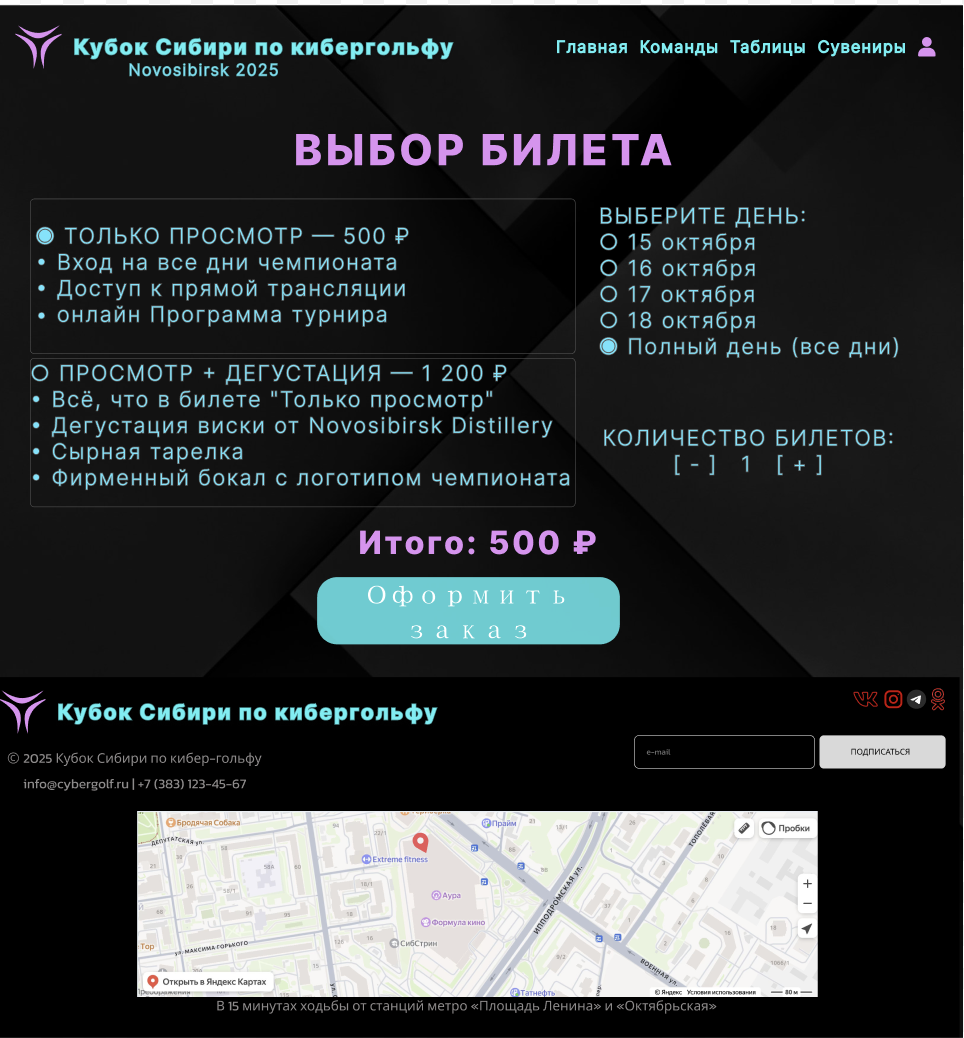
\includegraphics[width=0.7\textwidth]{photo/2.png}
    \caption{Детальная карточка билета с выбором типа (просмотр / просмотр+дегустация)}
\end{figure}

\begin{figure}[H]
    \centering
    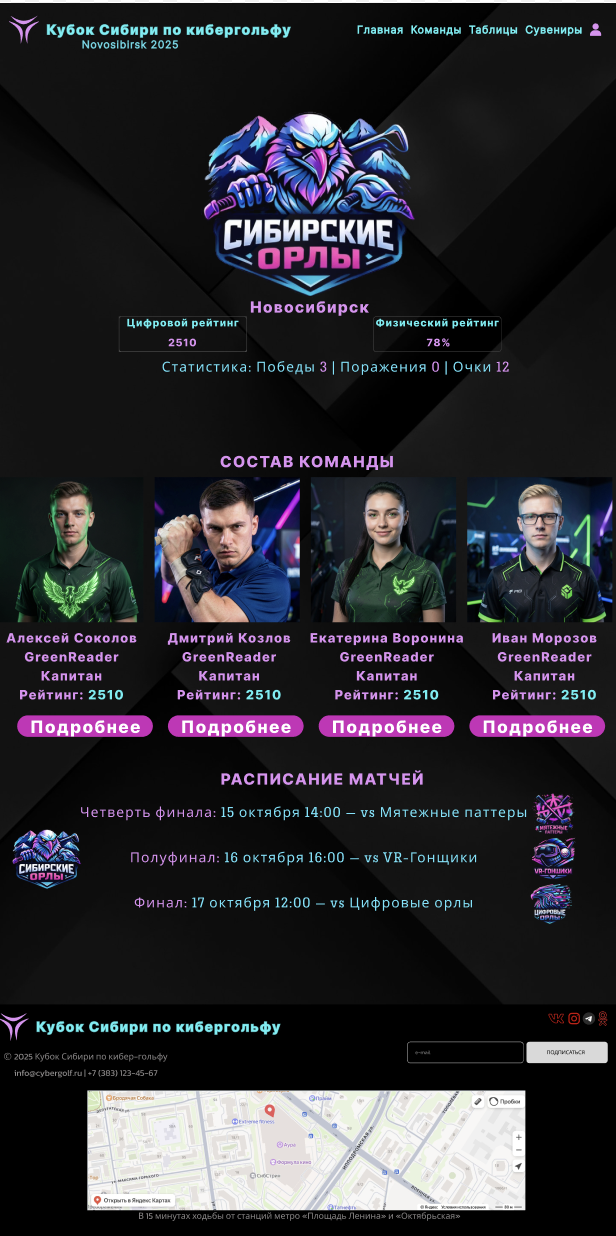
\includegraphics[width=0.7\textwidth]{photo/3.png}
    \caption{Страница команды "Сибирские Орлы" с карточками участников}
\end{figure}

\begin{figure}[H]
    \centering
    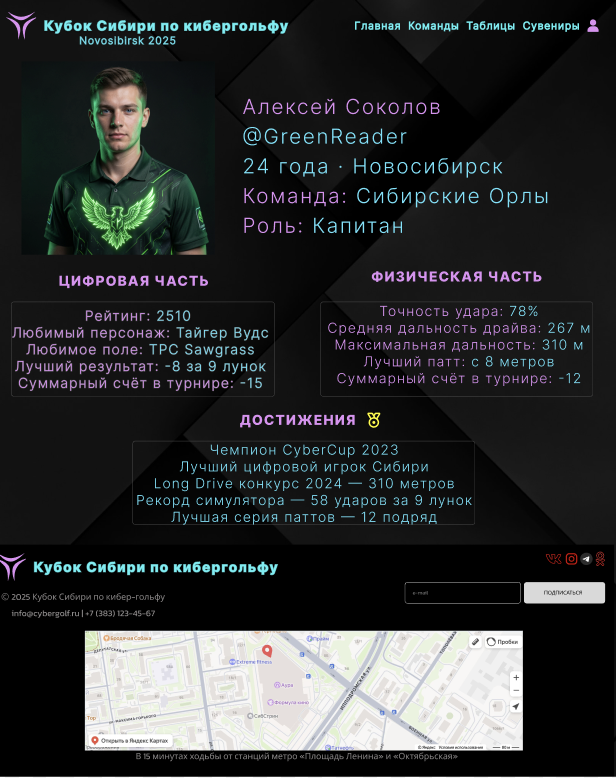
\includegraphics[width=0.7\textwidth]{photo/4.png}
    \caption{Карточка участника (Алексей "GreenReader" Соколов)}
\end{figure}

\begin{figure}[H]
    \centering
    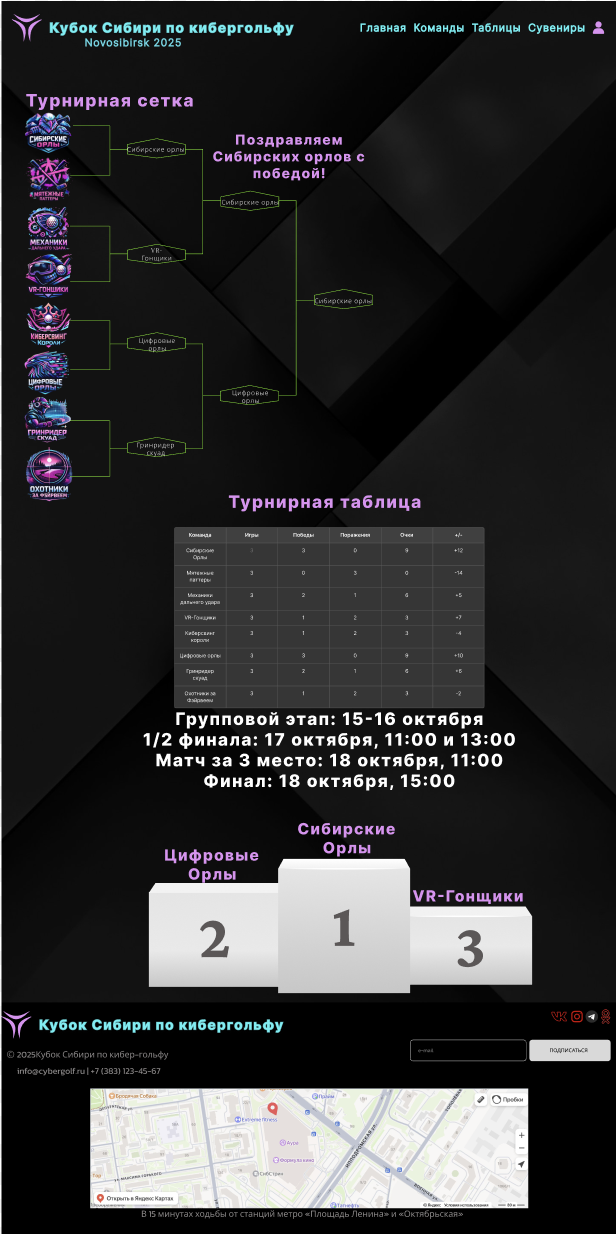
\includegraphics[width=0.7\textwidth]{photo/5.png}
    \caption{Турнирная таблица и сетка}
\end{figure}

\begin{figure}[H]
    \centering
    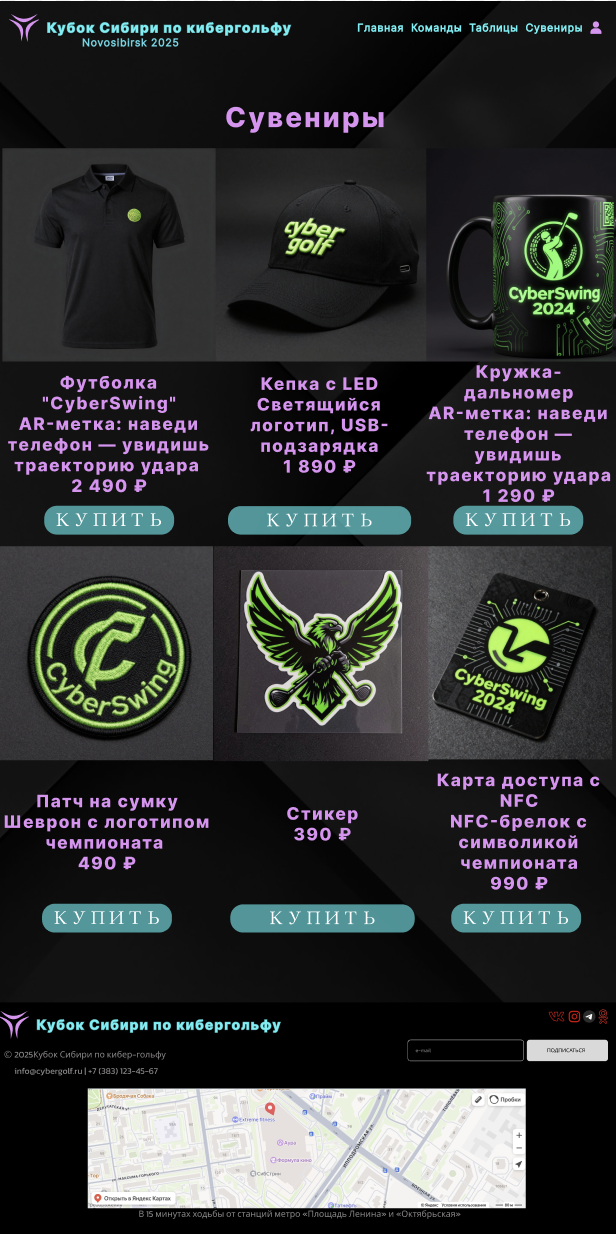
\includegraphics[width=0.7\textwidth]{photo/6.png}
    \caption{Каталог сувенирной продукции с символикой чемпионата}
\end{figure}

\begin{figure}[H]
    \centering
    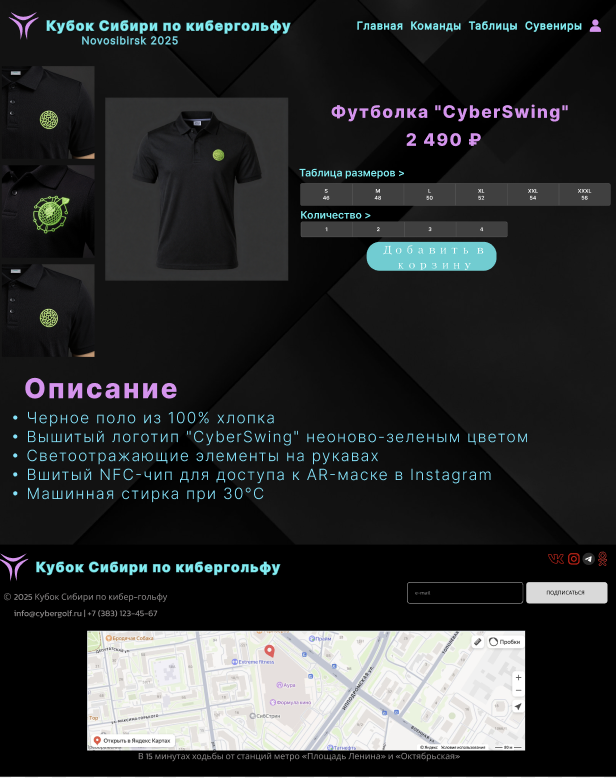
\includegraphics[width=0.7\textwidth]{photo/7.png}
    \caption{Детальная карточка футболки (выбор размера, количества, добавление в корзину)}
\end{figure}

\begin{figure}[H]
    \centering
    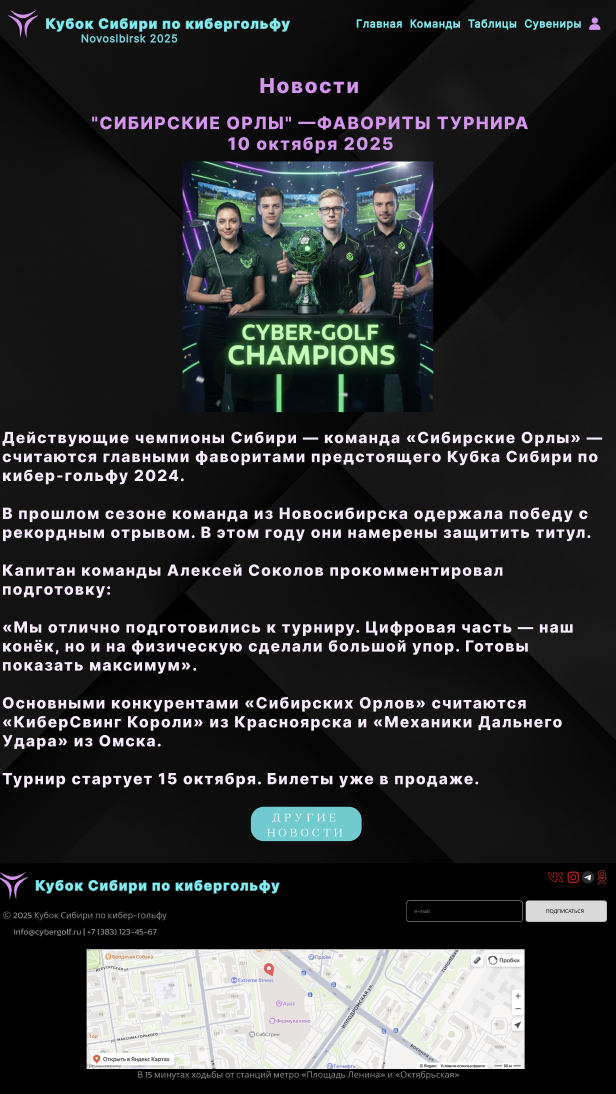
\includegraphics[width=0.7\textwidth]{photo/8.png}
    \caption{Страница новости о фаворитах турнира}
\end{figure}

\newpage
\subsection*{Ссылка на макет в Figma}

Работа доступна по ссылке: \\
\href{https://www.figma.com/design/k1NNNoWsYp2oCXssxQom8d/Untitled?node-id=87-1421&t=gqiGXhdBt5NyIpZ0-1}{Макет сайта чемпионата по кибер-гольфу "Кубок Сибири 2025"}

\section*{Заключение}
\addcontentsline{toc}{section}{Заключение}

В ходе выполнения практической работы был разработан дизайн сайта для чемпионата по фиджитал-спорту (кибер-гольф). Были выполнены следующие задачи:

\begin{enumerate}
    \item Разработана главная страница с информацией о турнире, списком из 8 команд, новостями, блоком продажи билетов и местом проведения
    \item Создана страница команды "Сибирскиде Орлы" с составом из 4 игроков (карточки участников)
    \item Разработана страница участника с разделением на цифровую и физическую части
    \item Построена турнирная таблица и сетка плей-офф
    \item Создан каталог сувенирной продукции с 6 товарами
    \item Реализована детальная карточка билета с выбором типа (просмотр / просмотр+дегустация)
    \item Добавлена детальная карточка товара (футболка) с выбором размера и количества
    \item Обеспечена адаптивность макета для трёх устройств: ПК (1440px), планшет (768px), мобильный телефон (360px)
\end{enumerate}
\end{document}